\section{系统设计}
\label{sec:system-design}

\add{当训练器与智能体脚手架解耦后，没有任何单一进程拥有完整的 rollout 生命周期：训练器拥有模型推理与优化，脚手架拥有上下文构建、控制流、工具使用与环境交互。智能体执行可能远程运行、超出任何单次 API 请求或 worker 进程的生命周期，且可能独立于训练进程失败。要将这一架构落地，需要一个轻量控制面来协调持久化 rollout 状态、外部执行、部分失败与资源使用，同时不把脚手架逻辑拉回训练器。}

\add{Agent Lightning v1.0 围绕声明式 rollout 抽象与调和循环（reconciliation loop）构建这一控制面。训练器通过 API 网关声明 rollout——网关是生命周期状态与只追加事件的唯一事实来源。Rollout 控制器持续将这一状态与运行于 Kubernetes Job 或本地进程的智能体执行进行调和。这种分离使 Kubernetes 成为可替换的执行后端，而非 rollout 抽象本身的一部分。}

\add{同一控制面还提供了跨服务边界的显式可靠性与可观测性语义。控制面操作幂等，生成尝试被显式记录与裁决，rollout 标识将模型请求、奖励、自定义事件与执行日志关联为一条诊断记录。最后，API 网关协调共址异步 RL 期间的推理准入，允许 rollout 与权重更新在无需向外部脚手架暴露相位切换的情况下分时共享同一 GPU 池。}

如图~\ref{fig:teaser} 所示，Agent Lightning v1.0 通过三个组件连接训练集群（运行模型推理与训练的 GPU 集群）与智能体执行集群。API 网关是一个 API 服务，存储 rollout、模型与事件，并将来自智能体脚手架的 LLM 调用转发到训练器注册的模型端点。Rollout 控制器在 Kubernetes 集群（或本地进程池）之上管理智能体执行，从 API 网关轮询 rollout 并启动相应智能体任务。定制化训练器基于 VERL~\cite{hybridflow} 构建，向 API 网关注册 rollout，等待 Rollout 控制器驱动其完成，然后取回其记录的事件组装训练样本。经由这一链路，训练器只创建 rollout 与收集轨迹；任何脚手架只需将其 LLM 端点切换到代理即可接入；训练与执行资源可以独立供给，甚至运行在不同地点。

Agent Lightning v1.0 的设计追求尽可能简单：整个系统约 3500 行代码实现，每个组件职责清晰。Agent Lightning v1.0 还内置了针对第~\ref{sec:challenges} 节挑战的设计选择，如 rollout 级奖励与优势计算、rollout 级损失归一化。

我们在附录~\ref{sec:appendix-system-design} 中详细描述每个组件，下文重点介绍若干特性。

\subsection{共址异步 RL}

智能体 RL 中，同步 RL 训练很慢：批次内所有 rollout 必须完成才能进行训练步更新，训练步必须等待批次中最慢的 rollout，使大量 GPU 空闲。AReaL~\cite{areal} 提出的异步 RL 将 rollout 与更新拆分到两个独立的机器池、各自占用不同 GPU，从而在更新运行时 rollout GPU 保持工作，解决了 GPU 空闲问题。但我们发现这总体上需要更多 GPU，对资源有限的小团队而言要求过高；且需要分别管理 rollout 队列与更新队列，实践中两个队列进度可能不同，管理更复杂。

\begin{figure}[t]
	\centering
	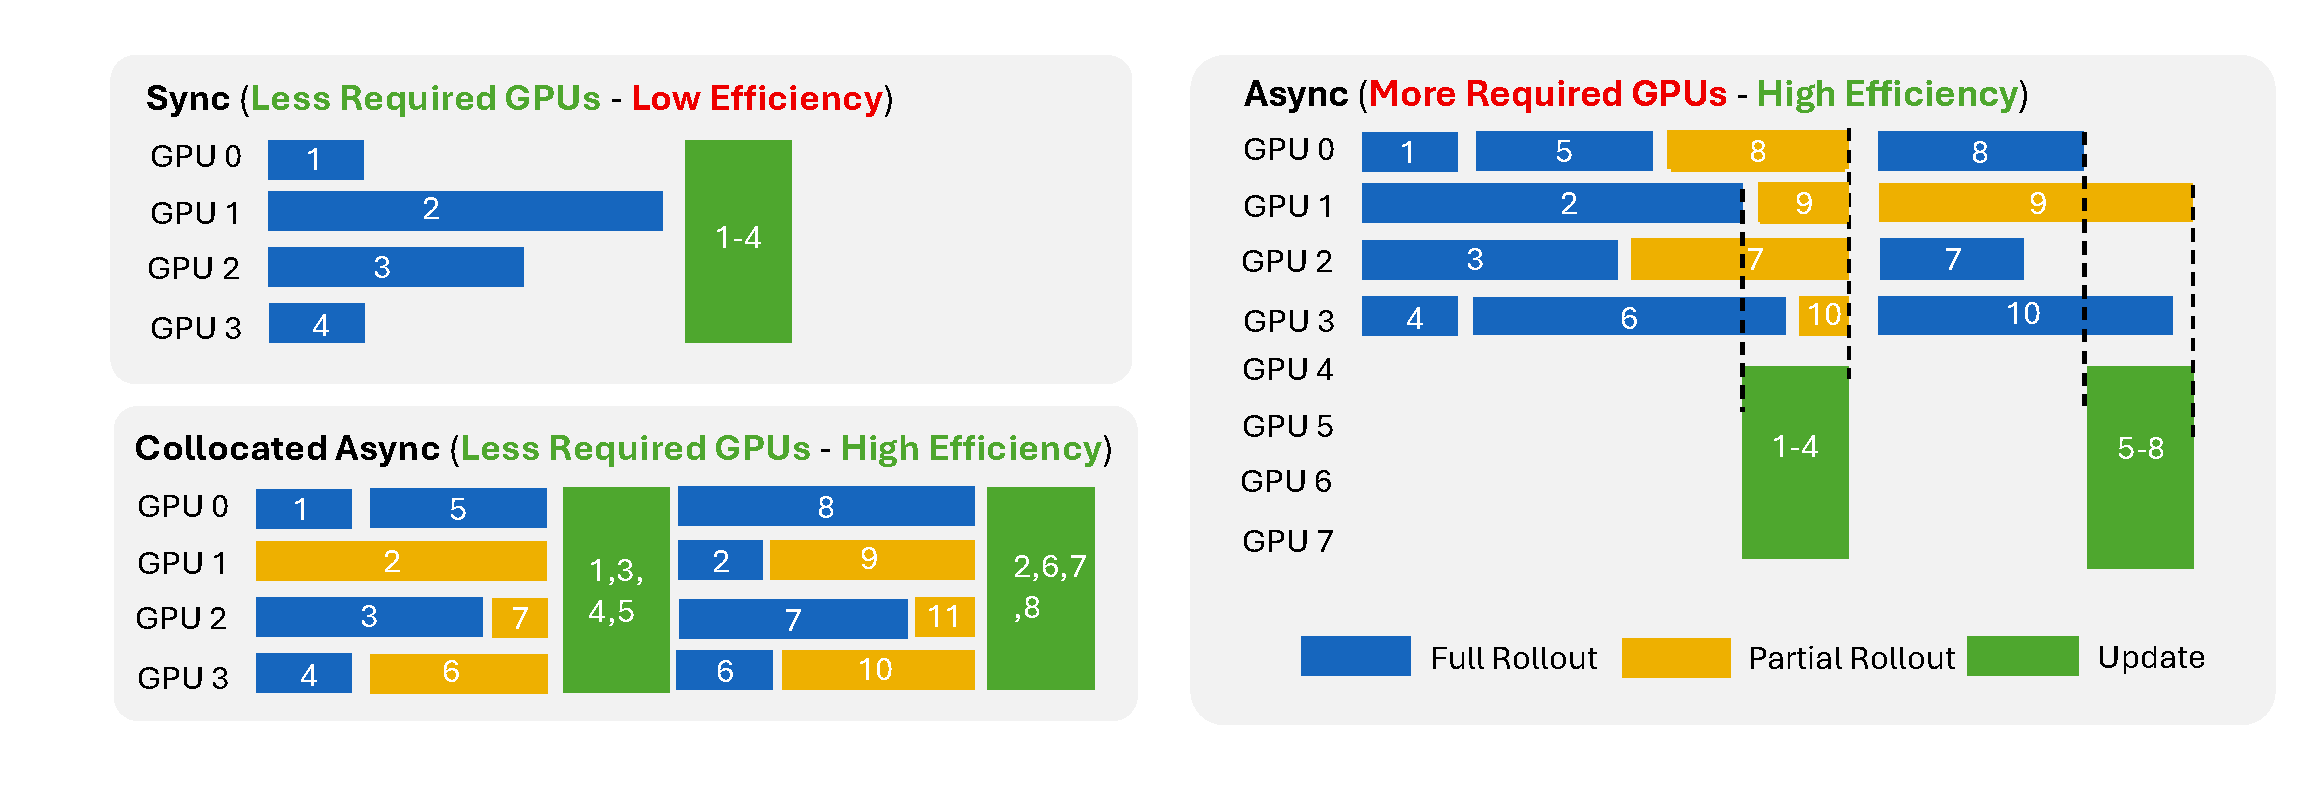
\includegraphics[width=\linewidth]{figures/agl-lite-async.pdf}
	\caption{同步 RL、异步 RL 与本文的共址异步 RL。共址异步 RL 在 rollout 与更新之间共享同一批 GPU，同时避免等待最慢的 rollout。}
	\label{fig:collocated-async}
\end{figure}

我们转而提出\emph{共址异步（collocated async）}，如图~\ref{fig:collocated-async} 所示。共址异步 RL 中，rollout 与权重更新共享同一 GPU 池。一旦收集到足够的 rollout 数据，更新步即开始。API 网关同时停止接受新请求并等待当前请求完成；此后若有新请求到达，网关将其暂停，直至系统重新进入 rollout 相位。因此，相位切换对智能体脚手架不可见。

共址异步让同一批 GPU 在 rollout 与训练之间分时共享，相比异步 RL 使用更少 GPU，同时避免等待最慢的 rollout。实验中，共址异步 RL 相比同步 RL 端到端加速约 2 倍，且使用更少 GPU。

\subsection{网络问题}

在\add{\harl{}}中，智能体与训练引擎分离，由此产生网络问题：两侧之间的调用经由网络传输，并非总是可靠。受影响的有两类调用：训练器或 Rollout 控制器到 API 网关的调用，以及智能体脚手架经代理到 LLM 推理端点的调用。两者都可能遭遇网络中断，调用方通常在失败后重试。我们用两项措施解决。

\paragraph{幂等的 API 网关端点。}我们将每个 rollout API 网关端点设计为幂等：重复同一调用任意次与调用一次效果相同。调用方因此在网络失败后可自由重试，无需担心重试本身破坏状态。

\paragraph{重复 LLM API 调用的去重。}重试的 LLM API 调用无法用同样方式幂等化，因为每次重试都是一次新的生成请求，可能返回不同响应。作为替代，定制化训练器在组装训练样本时对共享同一 prompt 的 \texttt{model\_request} 事件去重：若一次 rollout 记录了多个 prompt 相同的调用，只保留最后一次（最新）调用，丢弃更早的、对应重试或被取代的调用。

\subsection{Kubernetes 集成}

RL 训练的 rollout 阶段需要大量智能体并发运行，需要可观的计算资源。现有\add{\harl{}}框架普遍转向商业沙箱服务来满足这一需求：如 verl Uni-Agent~\cite{uniagent} 在 Modal Sandbox 与 Volcano veFaas 等托管沙箱上启动智能体执行，slime~\cite{slime} 依赖 E2B。这些服务提供便捷的开箱即用沙箱，但在 RL 训练规模下可能昂贵。

Agent Lightning v1.0 转而通过 Rollout 控制器直接在 Kubernetes 集群上运行智能体。每次智能体执行被调度为标准 Kubernetes Job，用户可完全依赖自托管或本地算力，而非商业沙箱提供商。这避免了商业沙箱服务的持续成本，并保持整个训练栈开源。

\subsection{监控}

训练期间，我们发现智能体自身可能出现问题，如奖励黑客、不良智能体行为与网络连接问题。人工检查 rollout 来发现这些问题很不方便，因此定制化训练器内置了监控系统，记录训练与验证 rollout 及 Kubernetes 的 pod 级日志，详见附录~\ref{sec:appendix-system-design}。该系统使我们能用 AI 智能体自动识别此类问题——我们确实借此发现了若干奖励黑客实例，见第~\ref{subsec:reward-hacking} 节。
